\documentclass[11pt]{article}
\usepackage{fullpage}
\usepackage{amsmath, amsfonts}
\usepackage{enumerate}
\usepackage{graphicx}

\title{CS4780/5780 Homework 6 Solutions}

\begin{document}
	\maketitle
	\section*{Problem 1: Optimization with Gradient Descent}
	\begin{enumerate}[(1)]
		\item[(a)] $f(w_5) = 80$
		\begin{center}
			\begin{tabular}{|c|c|}
				\hline
				$i$ & $w_i$ \\
				\hline
				0 & 13 \\
				1 & 9 \\
				2 & 13 \\
				3 & 9 \\
				4 & 13 \\
				5 & 9 \\
				\hline
			\end{tabular}
		\end{center}
		\item[(b)] $~$
		\begin{center}
			\begin{tabular}{|c|c|}
				\hline
				$i$ & $w_i$ \\
				\hline
				0 & 13 \\
				1 & 11 \\
				\hline
			\end{tabular}
		\end{center}
		\item[(c)] With $\alpha = \frac{1}{20}$, gradient descent won't converge - it will diverge. With $\alpha = \frac{1}{60}$, gradient descent starts at 13, then goes to 10 and a third, then increases gradually towards 11 in small increments, without ever exceeding 11. Solution should look something like below.
		\begin{center}
			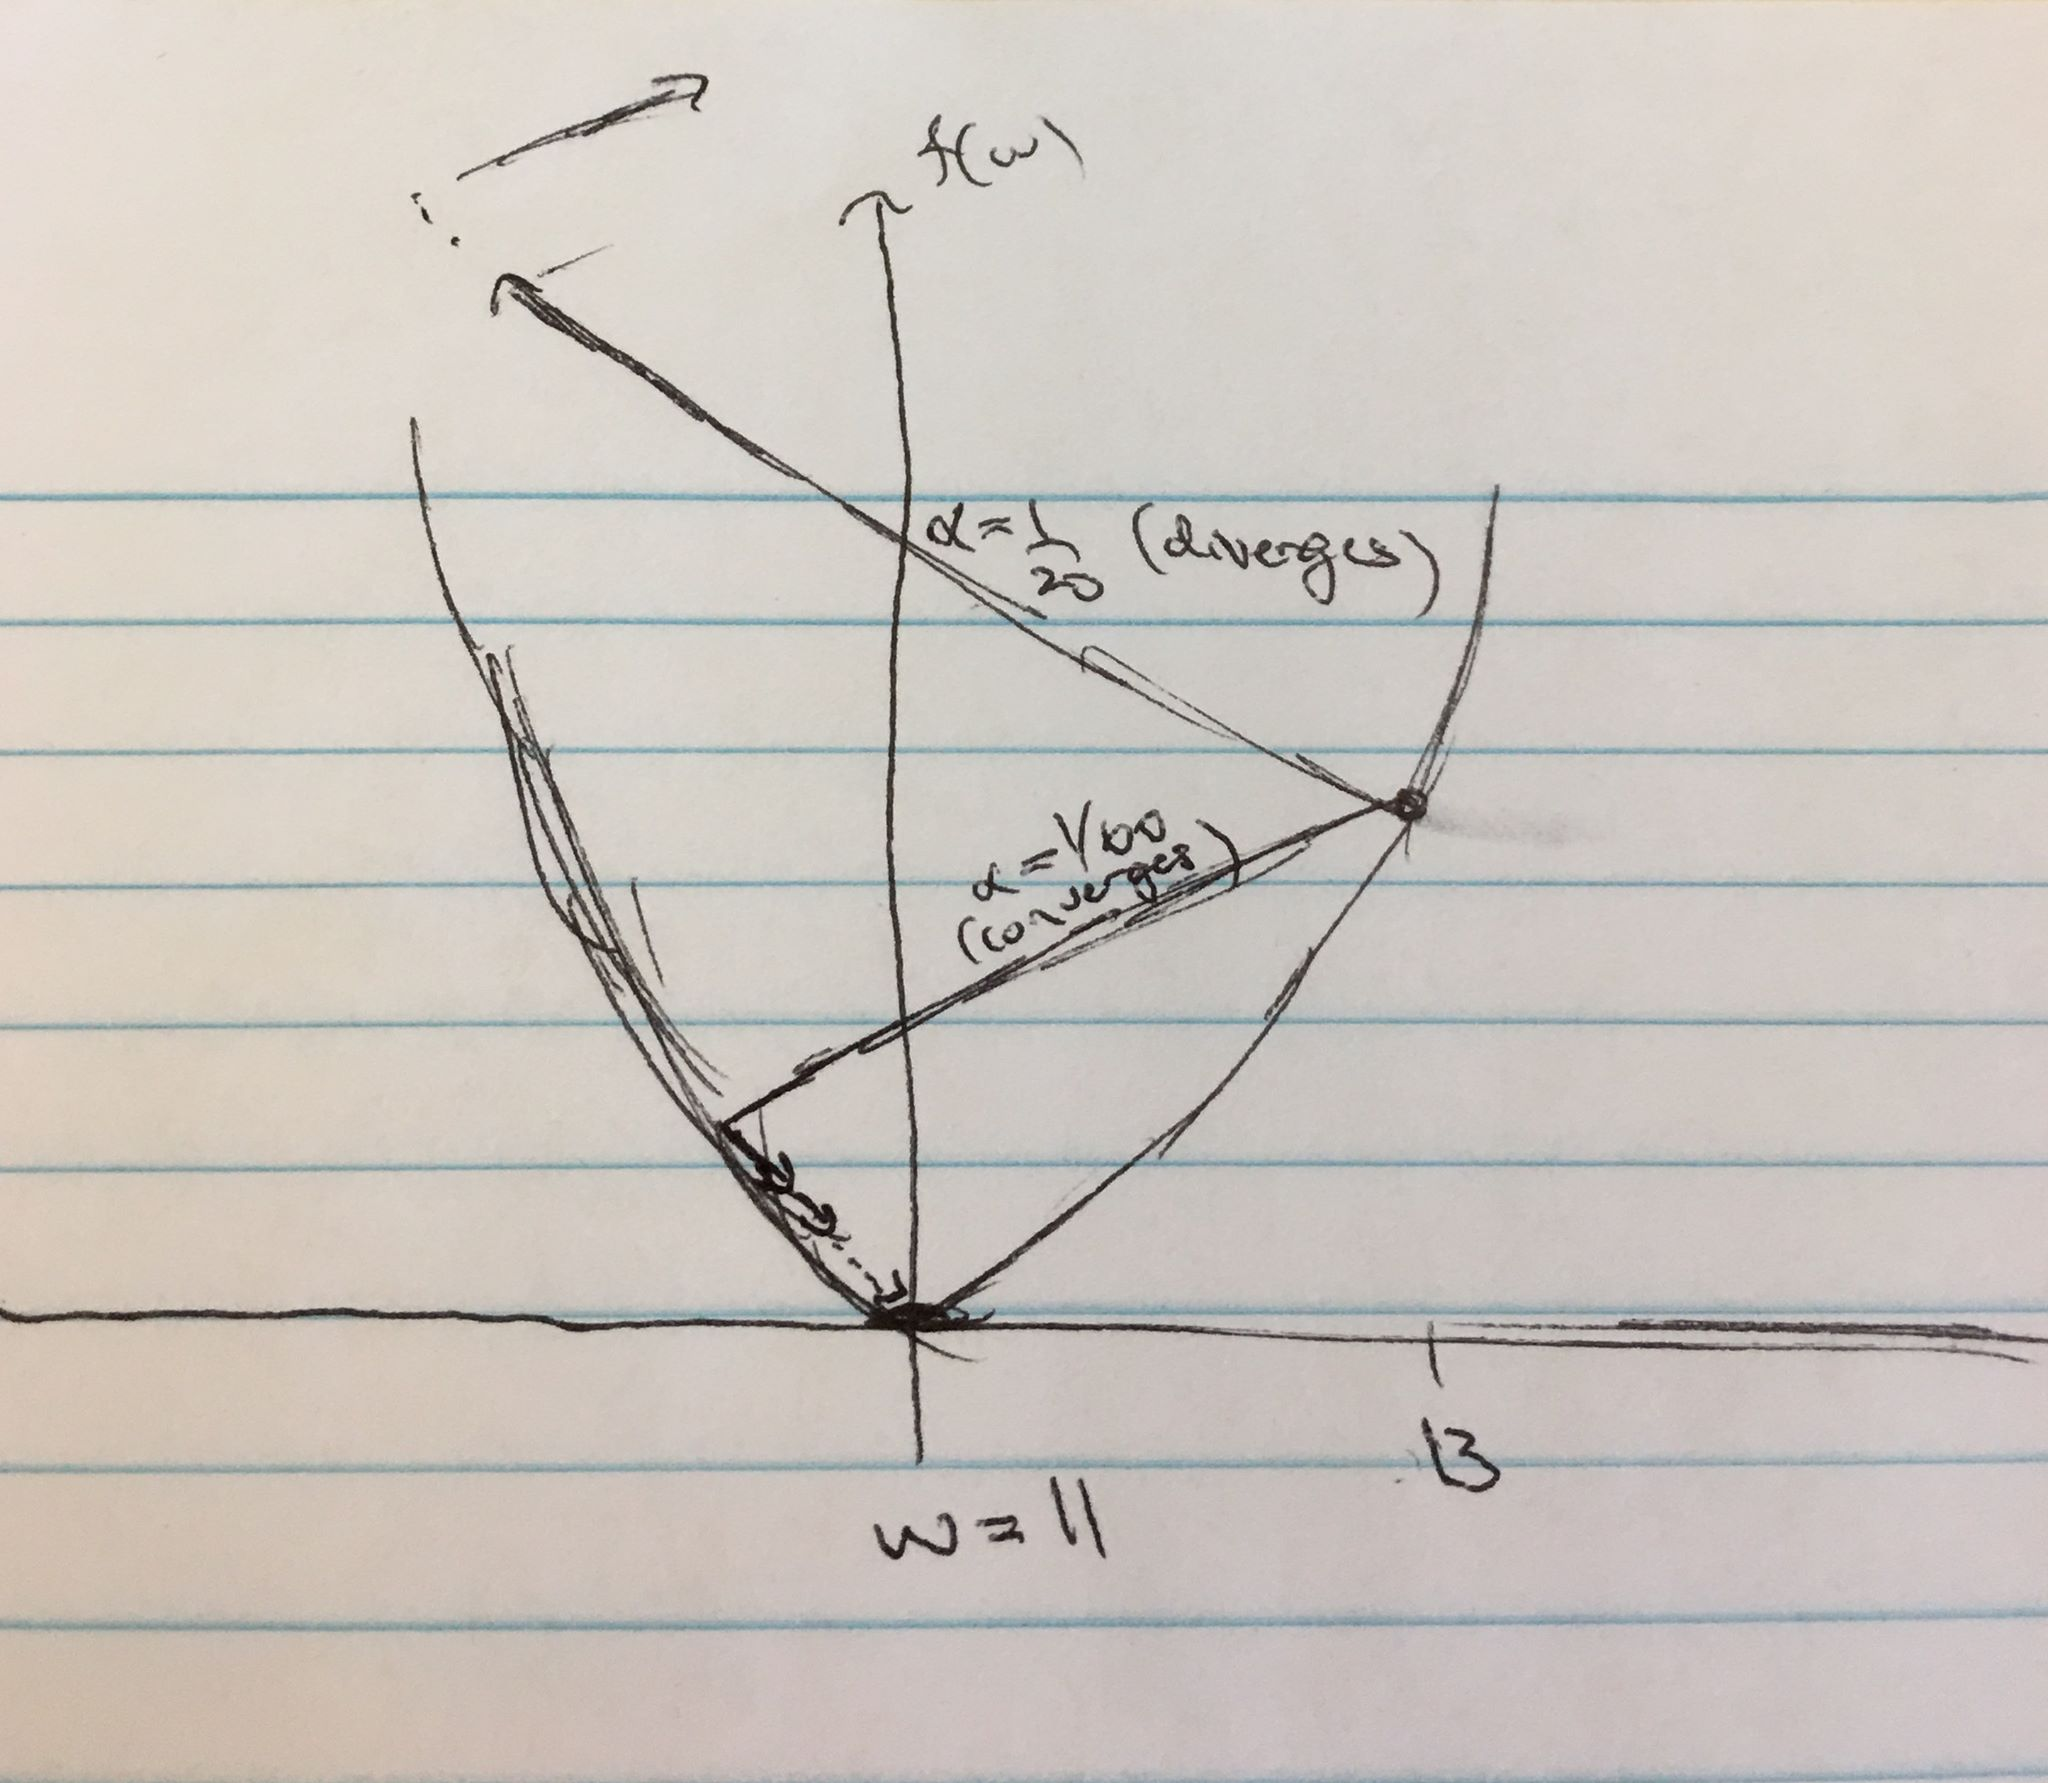
\includegraphics[scale=0.2]{1c}
		\end{center}
	\end{enumerate}
	\section*{Problem 2: Linear Regression}
	\begin{enumerate}[(1)]
		\item[(a)] Consider we have the following 1-d training set:
		\begin{center}
			
			\begin{tabular}{|c|c|}
				\hline
				$x$ & $y$ \\
				\hline
				-2 & 7 \\
				-1 & 4 \\
				0 & 3 \\
				1 & 4 \\
				2 & 7 \\
				\hline
			\end{tabular}
		\end{center}
		and our goal is to find a regression model that could regress $x$ to our target value $y$. To do this, we are going to use a linear regression model. Namely, we are going to model our data by assuming the relationship
		\begin{align*}
		y &= w_1x + w_0 + \epsilon \\
		&= \vec{w}^T\phi(x) + \epsilon
		\end{align*}
		where $\phi(x) = [1, x]^T$. We call $\phi$ a feature mapping of $x$ and this feature mapping allows us to absorb the bias $w_0$ into the vector $\vec{w}$.
		\begin{enumerate}[(1)]
			\item With this feature mapping, we can write down the design matrix as
			$$X = [\phi(x_1) ... \phi(x_n)]$$
			Using the formula given in class, compute the closed form solution for $\vec{w}$. Even though you are not required to calculate the inverse by hand, we strongly encourage you to do so since we expect you to be able to calculate the inverse of a $2 \times 2$ and $3 \times 3$ matrix by hand.
			\newline \\
			\textbf{Solution} From class, $$\vec{w}=(XX^\top)^{-1}X\vec{y}^\top$$.
			We are given,
			\begin{align*}
			X = \begin{bmatrix}
			1 & 1 & 1 &1 & 1           \\[0.3em]
			-2 & -1 & 0 &1 &2
			\end{bmatrix},\,
			\vec{y} = \begin{bmatrix}
			7 \\[0.3em]
			4 \\
			3 \\
			4 \\
			7
			\end{bmatrix}
			\end{align*}
			Hence,
			\begin{align*}
			XX^\top & = \begin{bmatrix}
			5 & 0          \\[0.3em]
			0 & 10
			\end{bmatrix} \\
			(XX^\top)^{-1} & = \begin{bmatrix}
			0.2 & 0          \\[0.3em]
			0 & 0.1
			\end{bmatrix}
			\end{align*}
			Remember, given $AA^{-1}=\textbf{I}$,
			\begin{align*}
			A^{-1} = \begin{bmatrix}
			a & b           \\[0.3em]
			c & d
			\end{bmatrix}^{-1} =
			\frac{1}{ad-bc}\begin{bmatrix}
			d & -b           \\[0.3em]
			-c & a
			\end{bmatrix}.
			\end{align*}
			Applying matrix multiplication, we find
			\begin{align*}
			\vec{w} = \begin{bmatrix}
			5           \\[0.3em]
			0
			\end{bmatrix}
			\end{align*}
			
			\item Recall that the loss function for linear regression is
			$$\ell(\vec{w}) = \sum_{i = 1}^{n} (y_i - \vec{w}^T \phi(x_i))^2$$
			With the closed formed solution obtained in (a)(1), calculate the training loss.
			\newline \\
			\textbf{Solution} Directly applying the loss function,
			\begin{align*}
			\ell(\vec{w}) & = \sum_{i = 1}^{5} (y_i - \vec{w}^T \phi(x_i))^2 \\
			& = (7 -
			\begin{bmatrix}
			5 & 0
			\end{bmatrix} \begin{bmatrix}
			1           \\[0.3em]
			-2
			\end{bmatrix})^2 + (4 -
			\begin{bmatrix}
			5 & 0
			\end{bmatrix} \begin{bmatrix}
			1           \\[0.3em]
			-1
			\end{bmatrix})^2 +...+ (7 -
			\begin{bmatrix}
			5 & 0
			\end{bmatrix} \begin{bmatrix}
			1           \\[0.3em]
			2
			\end{bmatrix})^2 \\
			& = 14.
			\end{align*}
		\end{enumerate}
		\item[(b)]
		In (a)(2), we realize that we could not attain a training loss of zero. It seems like the $y$ is a quadratic function of $x$, instead of a linear function of $x$. Now, let us define a new feature mapping $\phi_2(x) = [1, x, x^2]$. With this new feature mapping, what is the closed form solution $\vec{w}$? Can we attain a training loss of zero with this closed form solution?
		\newline \\
		\textbf{Solution} Using the same process as before,
		\begin{align*}
		X = \begin{bmatrix}
		1 & 1 & 1 & 1 & 1   \\[0.3em]
		-2 & -1 & 0 & 1 & 2 \\[0.3em]
		4 & 1 & 0 & 1 & 4
		\end{bmatrix},\,
		\vec{y} = \begin{bmatrix}
		7 \\[0.3em]
		4 \\
		3 \\
		4 \\
		7
		\end{bmatrix}
		\end{align*}
		Hence,
		\begin{align*}
		XX^\top & = \begin{bmatrix}
		5 & 0 & 10 \\[0.3em]
		0 & 10 & 0 \\[0.3em]
		10 & 0 & 34
		\end{bmatrix} \\
		(XX^\top)^{-1} & = \begin{bmatrix}
		0.486 & 0 & -0.143 \\[0.3em]
		0 & 0.1 & 0        \\[0.3em]
		-0.143 & 0 & 0.071
		\end{bmatrix}
		\end{align*}
		Applying matrix multiplication, we find
		\begin{align*}
		\vec{w} = \begin{bmatrix}
		3 \\[0.3em]
		0 \\[0.3em]
		1
		\end{bmatrix}
		\end{align*}.
		Directly applying the loss function,
		\begin{align*}
		\ell(\vec{w}) & = \sum_{i = 1}^{5} (y_i - \vec{w}^T \phi_2(x_i))^2 \\
		& = 0.
		\end{align*}
	\end{enumerate}
	\textbf{Take-away:} Feature extraction is essential in creating a powerful model. Although we will not cover how to design hand-crafted features, we will cover how to automatically learn a powerful representation of the data using kernel methods and possibly deep learning if time permits.
	\section*{Problem 3: Weighted Ridge Regression}
	Suppose we have a dataset $\{(\vec{x}_1, y_1), ..., (\vec{x}_n, y_n)\}$. In a ridge regression setting, we assume that each example is equally important. Sometimes, certain examples are more important than others and we would want to assign a positive weight $p_i$ to each training examples to indicate the level of importance of each training example. For instance, in the previous problem, if we care more about the predictions of our model on the examples with positive $x$, then we might assign higher weights to those training examples with positive $x$ than those training examples with negative $x$.
	\newline
	\newline
	In order to modify ridge regression to account for the weights of different training examples, we rewrite the loss function as
	$$\ell(\vec{w}) = \sum_{i = 1}^{n}(p_i(\vec{w}^T\vec{x}_i - y_i)^2) + \lambda \vec{w}^T \vec{w}$$ where $\lambda \geq 0$.
	\begin{enumerate}[(1)]
		\item[(1)] Suppose $X = [\vec{x}_1, ..., \vec{x}_n]^T$, $\vec{y} = [y_1, ..., y_n]^T$. Find a diagonal matrix P such that we can rewrite the loss function as $$\ell(\vec{w}) =  (X\vec{w} - \vec{y})^TP(X\vec{w} - \vec{y}) + \lambda \vec{w}^T \vec{w}$$
		\newline
		\newline
		\textbf{Solution}
		We are looking for the diagonal matrix $P$ in terms of elements $p_i$
		\newline
		In order to do this we create matrix $P$ with elements $p_{ij}$ such that:
		\newline
		$$p_{ij} = 
		\begin{cases} 
		p_i & i = j \\
		0 & \text{otherwise} \\ 
		\end{cases}		
		$$
		
		\item[(2)] Using the rewritten loss function, derive a closed form solution for $\vec{w}$ by setting the gradient of the loss function equal to zero.
		\newline
		\newline
		\textbf{Solution}
		\begin{align*}
		\ell(\vec{w}) &= (X\vec{w} - \vec{y})^TP(X\vec{w} - \vec{y}) + \lambda \vec{w}^T \vec{w} \\
		&= \vec{w}^TX^TPX\vec{w} - \vec{w}^TX^TP\vec{y}- \vec{y}^TPX\vec{w} + \vec{y}^T\vec{y} + \lambda \vec{w}^T \vec{w} \\
		&= \vec{w}^TX^TPX\vec{w} - 2\vec{w}^TX^TP\vec{y} + \vec{y}^T\vec{y} + \lambda \vec{w}^T \vec{w} \\
		\end{align*}
		We take the gradient and set it equal to 0
		\begin{align}
		\nabla_w \ell = 2(X^TPX)\vec{w} - 2(X^TP)\vec{y} +2\lambda\vec{w} = 0
		\end{align}
		Using some algebra very similar to that shown in class when deriving the closed form for ridge regression, we get:
		\begin{align}
		\vec{w} = (X^TPX + \lambda I)^{-1}(X^TP)\vec{y}
		\end{align}
		\item[(3)] Show that the loss function is convex by showing the $\nabla^2 \ell$ is positive semidefinite for any $\vec{w}$. By showing the loss function is convex, we can conclude that the closed formed we derived in (2) is indeed a global minimum point.
		\newline
		\newline
		\textbf{Solution} We find the hessian of $\ell(\vec{w})$
		\begin{align*}
		\nabla^2_{\vec{w}} \ell = 2 (X^TPX + \lambda I)
		\end{align*}
		An $n \times n$ symmetric matrix $A$ is positive semidefinite if for any non-zero $n \times1$ vector, $\vec{z}$, the following is true:
		\begin{align*}
		\vec{z}^TA\vec z \geq 0
		\end{align*}
		We see that both $(X^TPX)$ and $\lambda I$ are both symmetric and as a result, their sum is also symmetric. Additionally, the sum of two positive semidefinite matrices is positive semidefinite since $\vec{z}^T(A+B)\vec z = \vec{z}^T(A)\vec z + \vec{z}^TB\vec z \geq 0 + 0 = 0$. So, if we can show that $\lambda I$ and $X^TPX$ are positive semidefinite, then we are done!
		\newline
		\newline
		Let's start with the $\lambda I$ term. Expanding $\vec{z}^T\lambda I\vec z$, we have 
		\begin{align*}
		\vec{z}^T\lambda I\vec z = \sum\limits_{i=1}^n \lambda z_i^2 \geq 0
		\end{align*}
		Because $\lambda$ is nonnegative, this sum will be nonnegative as well. Now for the $X^TPX$ term, we have
		\begin{align*}
		\vec{z}^TX^TPX\vec z = (Xz)^TP(Xz)
		= \sum\limits_{i=1}^n p_{ii} * (x_{i}z)^2 \geq 0
		\end{align*}
		\newline
		We see that P is a diagonal matrix with positive values so this sum must also be nonnegative.
		Therefore, $\nabla^2_{\vec{w}} \ell$ is positive semidefinite.
	\end{enumerate}
	
	
	
\end{document}
